\documentclass{article}

\usepackage[latin1]{inputenc}
\usepackage{pgfplots}
\usepackage{tikz}
\usetikzlibrary{arrows}

\pgfplotsset{compat=1.10}

\begin{document}
\pagestyle{empty}

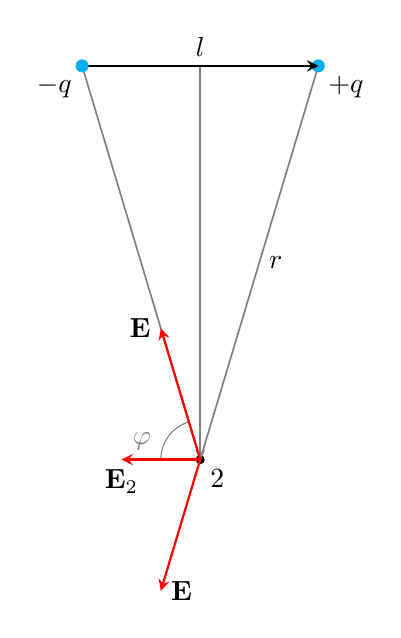
\begin{tikzpicture}[>=stealth]
	\draw[fill] (0, -5) circle [radius=0.05];
	\draw[gray, semithick, ->] (0, 0) -- (0, -5) node[black, below right] {2};
	\draw[gray, semithick] (0, -5) -- (-1.5, 0);
	\draw[gray, semithick] (0, -5) -- (1.5, 0);

	\draw[cyan, fill] (1.5, 0) circle [radius=0.075];
	\draw[-latex, thick, ->] (-1.5, 0) node[below left] {$-q$} -- (1.5, 0) node[below right] {$+q$};
	\draw[cyan, fill] (-1.5, 0) circle [radius=0.075];
	\node[above] at (0, 0) {$l$};
	\node[right] at (0.75, -2.5) {$r$};

	\draw[gray] ([shift=(106.6993:0.5cm)]0, -5) arc (106.6993:180:0.5cm) node[above left] {$\varphi$};

	\draw[red, thick, ->] (0, -5) -- (-0.5, -3.3334) node[black, left] {$\textbf{E}$};
	\draw[red, thick, ->] (0, -5) -- (-0.5, -6.6667) node[black, right] {$\textbf{E}$};
	\draw[red, thick, ->] (0, -5) -- (-1, -5) node[black, below] {$\textbf{E}_2$};
\end{tikzpicture}

\end{document}